\documentclass[tikz,border=2pt]{standalone}
\usepackage{amsmath}
\usetikzlibrary{arrows.meta,matrix,calc}
\begin{document}
% Row reduction of A (3x4, rank 2) to R keeps the row space: the nonzero rows of R are a basis of
% Row(A), and row 3 of A is row 1 + row 2. The column space is read from the pivot columns 1, 3 of A.
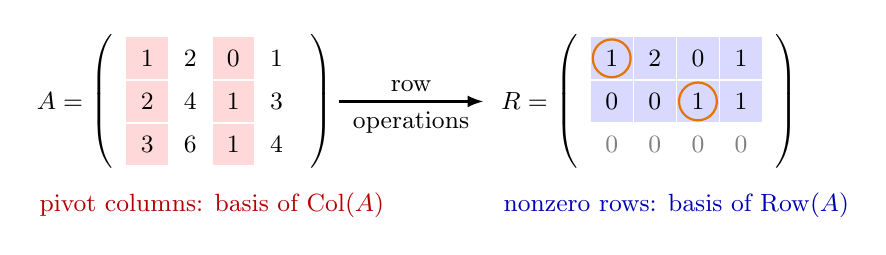
\begin{tikzpicture}[font=\small, >={Latex[length=2mm]},
  m/.style={matrix of math nodes, nodes={minimum width=5.3mm, minimum height=5.3mm, anchor=center},
    left delimiter=(, right delimiter=), column sep=0.5pt, row sep=0.5pt}]
  \matrix (A) [m] at (0,0) {
    |[fill=red!15]| 1 & 2 & |[fill=red!15]| 0 & 1 \\
    |[fill=red!15]| 2 & 4 & |[fill=red!15]| 1 & 3 \\
    |[fill=red!15]| 3 & 6 & |[fill=red!15]| 1 & 4 \\
  };
  \node[anchor=east] at ([xshift=-3mm]A.west) {$A=$};
  \matrix (R) [m] at (5.9,0) {
    |[fill=blue!15]| 1 & |[fill=blue!15]| 2 & |[fill=blue!15]| 0 & |[fill=blue!15]| 1 \\
    |[fill=blue!15]| 0 & |[fill=blue!15]| 0 & |[fill=blue!15]| 1 & |[fill=blue!15]| 1 \\
    |[text=gray]| 0 & |[text=gray]| 0 & |[text=gray]| 0 & |[text=gray]| 0 \\
  };
  \node[anchor=east] (Rl) at ([xshift=-3mm]R.west) {$R=$};
  \draw[->, thick] ([xshift=4mm]A.east) -- ([xshift=-1mm]Rl.west)
    node[midway, above] {row} node[midway, below] {operations};
  % pivots of R (columns 1 and 3)
  \draw[orange!90!black, thick] (R-1-1) circle (2.4mm);
  \draw[orange!90!black, thick] (R-2-3) circle (2.4mm);
  % annotations
  \node[red!70!black, anchor=north] at ([yshift=-1mm]A.south) {pivot columns: basis of $\operatorname{Col}(A)$};
  \node[blue!70!black, anchor=north] at ([yshift=-1mm]R.south) {nonzero rows: basis of $\operatorname{Row}(A)$};
\end{tikzpicture}
\end{document}
